\documentclass{article}

% Document extensibility %
%
% Disables native paragraph indentation
\usepackage{parskip} 
%
% Provides further bullet options for lists
\usepackage{enumitem}

% Mathematical symbol and statement packages %
%
% Necessary
\usepackage{amsmath}
\usepackage{amssymb}
%
% Extensive fraction notation
\usepackage{xfrac}
%
% Generic mathematical commands
% Notable: \degree, \celcius
\usepackage{gensymb}
%
% Variable vector notation (arrow above variable)
\usepackage{esvect}
%
% Multiline boxed equations
\usepackage{empheq}
%
% SI Unit
\usepackage{siunitx}
\usepackage{physunits}
%
% More intuitive arrays/matrices
\usepackage{array}
%
% Linear Equations
\usepackage{systeme}
%
% Boxes!
\usepackage{mdframed}
%
% Matrix Notation
\usepackage{bm}

% Graphic packages %
%
% Diagrams and illustrations
\usepackage{tikz}
\usetikzlibrary{positioning}
%
% Image insertion
\usepackage{graphicx}

% Document content %
%
% Change title of table of contents
% \renewcommand{\contentsname}{Title}

\title{Homework 8 - Momentum}
\author{Corey Mostero - 2566652}
\date{25 May 2023}

\begin{document}

% Command `\hr` to insert horizontal rules
\newcommand{\hr}{\par\noindent\rule{\textwidth}{0.4pt}}

% Command to box and center math equations
\newcommand{\bc}[1]{
	\begin{equation*}
		\begin{boxed}
			{#1}
		\end{boxed}
	\end{equation*}
}

% Command for single line equations with a condition
\newcommand{\cond}[2]{
	\ifmmode
		{#1} \quad {#2}
	\else
		$$ {#1} \quad {#2} $$
	\fi
}

% Matrix and Vector notation
\newcommand{\matr}[1]{
	\ifmmode \bm{#1}
	\else \textit{\textbf{#1}}
	\fi
}
\newcommand{\vect}[1]{
	\ifmmode \mathbf{#1}
	\else \textbf{#1}
	\fi
}

\maketitle
\newpage

\tableofcontents

\section{Book}

\subsection{8.16}

\begin{align*}
	m_{(a)stronaut} & = \SI{65.5}{\kilogram} \\
	m_{(t)ool} & = \SI{2.50}{\kilogram} \\
	v_{t_1} & = \SI{3.10}{\meter \per \second} \\
	v_{a_1} & = ?
\end{align*}
\begin{align*}
	P_0 & = P_1 \\
	m_av_{a_0} + m_tv_{t_0} & = m_av_{a_1} + m_tv_{t_1} \\
	0 + 0 & = m_av_{a_1} + m_tv_{t_1} \\
	v_{a_1} & = -\frac{m_tv_{t_1}}{m_a} \\
	v_{a_1} & = -\frac{(\SI{2.50}{\kilogram})(\SI{3.10}{\meter \per \second})}{\SI{65.5}{\kilogram}} \\
	v_{a_1} & = \SI{-0.118}{\meter \per \second}
\end{align*}
\begin{mdframed}
	The astronaut will move at a speed of \SI{0.118}{\meter \per \second} opposite of the tool's direction.
\end{mdframed}

\subsection{8.21}

\begin{align*}
	m_A & = \SI{0.245}{\kilogram} \\
	m_B & = \SI{0.360}{\kilogram} \\
	v_{B_0} & = 0 \\
	v_{A_1} & = \SI{-0.118}{\meter \per \second} \\
	v_{B_1} & = \SI{0.660}{\meter \per \second} \\
	v_{A_0} & = ?
\end{align*}
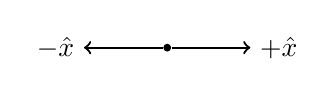
\begin{tikzpicture}
	\node [circle, fill, inner sep = 1pt] (origin) {};
	\node [left = of origin] (x0) {$ -\hat{x} $};
	\node [right = of origin] (x1) {$ +\hat{x} $};

	\foreach \node in {x0, x1}
		\draw[black, thick, ->] (origin) -- (\node);
\end{tikzpicture}
\begin{enumerate}[label = \textbf{(\alph*)}]
	\item What was the speed of puck $ A $ before the collision?
		\begin{align*}
			P_0 & = P_1 \\
			m_A v_{A_0} + m_B v_{B_0} & = m_A v_{A_1} + m_B v_{B_1} \\
			m_A v_{A_0} + 0 & = m_A v_{A_1} + m_B v_{B_1} \\
			v_{A_0} & = \frac{ m_A v_{A_1} + m_B v_{B_1} }{ m_A } \\
			v_{A_0} & = \frac{ (\SI{0.245}{\kilogram})(\SI{-0.118}{\meter \per \second}) + (\SI{0.360}{\kilogram})(\SI{0.660}{\meter \per \second}) }{ \SI{0.245}{\kilogram} } \\
			v_{A_0} & = \SI{0.852}{\meter \per \second}
		\end{align*}
		\bc{ v_{A_0} = \SI{0.852}{\meter \per \second} }
	\item Calculate the change in the total kinetic energy of the system that occurs during the collision.
		\begin{align*}
			\Delta PE & = E_{A_1} + E_{B_1} - E_{A_0} + E_{B_0} \\
			\Delta PE & = \frac{1}{2}m_Av_{A_1}^2 + \frac{1}{2}m_Bv_{B_1}^2 - \frac{1}{2}m_Av_{A_0}^2 + 0 \\
			\Delta PE & = \frac{1}{2}(\SI{0.245}{\kilogram})(\SI{-0.118}{\meter \per \second})^2 + \frac{1}{2}(\SI{0.360}{\kilogram})(\SI{0.660}{\meter \per \second})^2 - \frac{1}{2}(\SI{0.245}{\kilogram})(\SI{0.852}{\meter \per \second})^2 \\
			\Delta PE & = \SI{-0.00881}{\joule} = \SI{8.81e-3}{\joule}
		\end{align*}
		\bc{ \Delta PE = \SI{-0.00881}{\joule} = \SI{8.81e-3}{\joule} }
\end{enumerate}

\subsection{8.30}

\begin{align*}
	m_A = m_B & = ? \\
	v_{A_0} & = \SI{40.0}{\meter \per \second} \\
	\theta_A & = \SI{30.0}{\degree} \\
	v_{B_0} & = 0 \\
	\theta_B & = \SI{-45.0}{\degree} \\
	v_{A_1} & = ? \\
	v_{B_1} & = ?
\end{align*}
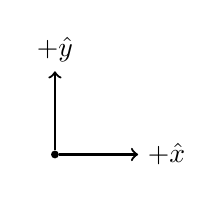
\begin{tikzpicture}
	\node [circle, fill, inner sep = 1pt] (origin) {};
	\node [above = of origin] (y) {$ +\hat{y} $};
	\node [right = of origin] (x) {$ +\hat{x} $};

	\foreach \node in {y, x}
		\draw[black, thick, ->] (origin) -- (\node);
\end{tikzpicture}
\begin{enumerate}[label = \textbf{(\alph*)}]
	\item Find the speed of each asteroid after the collision. \\
		Speed of asteroid in $ \hat{x} $ direction:
		\begin{align*}
			v_{A_0} & = \SI{40.0}{\meter \per \second}\cos(\SI{0}{\degree}) = \SI{40.0}{\meter \per \second} \\
			v_{B_0} & = 0 \\
			v_{A_1} & = v_{A_1}\cos(\SI{30.0}{\degree}) \\
			v_{B_1} & = v_{B_1}\cos(\SI{-45.0}{\degree})
		\end{align*}
		\begin{align*}
			P_{0_x} & = P_{1_x} \\
			m_Av_{A_0} + m_Bv_{B_0} & = m_Av_{A_1} + m_Bv_{B_1} \\
			v_{A_0} & = v_{A_1} + v_{B_1} \\
			\SI{40.0}{\meter \per \second} & = v_{A_1}\cos(\SI{30.0}{\degree}) + v_{B_1}\cos(\SI{-45.0}{\degree})
		\end{align*}
		Speed of asteroid in $ \hat{y} $ direction:
		\begin{align*}
			v_{A_0} & = \SI{40.0}{\meter \per \second}\cos(\SI{90}{\degree}) = 0 \\
			v_{B_0} & = 0 \\
			v_{A_1} & = v_{A_1}\sin(\SI{30.0}{\degree}) \\
			v_{B_1} & = v_{B_1}\sin(\SI{-45.0}{\degree})
		\end{align*}
		\begin{align*}
			P_{0_y} & = P_{1_y} \\
			m_Av_{A_0} + m_Bv_{B_0} & = m_Av_{A_1} + m_Bv_{B_1} \\
			0 & = v_{A_1} + v_{B_1} \\
			v_{A_1}\sin(\SI{30.0}{\degree}) + v_{B_1}\sin(\SI{-45.0}{\degree}) & = 0
		\end{align*}
		\begin{align*}
			\left[ \matr{A} | \vect{v} \right] & =
				\left[ \begin{array}{ c c | c }
					\cos(\SI{30.0}{\degree}) & \cos(\SI{-45.0}{\degree}) & \SI{40.0}{\meter \per \second} \\
					\sin(\SI{30.0}{\degree}) & \sin(\SI{-45.0}{\degree}) & 0
			\end{array} \right]
		\end{align*}
		\begin{align*}
			\matr{A}_2 & = \matr{A}_2 - \matr{A}_1 \frac{\sqrt{3}}{3} \\
			\left[ \matr{A} | \vect{v} \right] & =
				\left[ \begin{array}{ c c | c }
					\cos(\SI{30.0}{\degree}) & \cos(\SI{-45.0}{\degree}) & \SI{40.0}{\meter \per \second} \\
					0 & -1.12 & \SI{-23.1}{\meter \per \second}
			\end{array} \right]
		\end{align*}
		\begin{align*}
			-1.12 \vect{v}_B & = \SI{-23.1}{\meter \per \second} \\
			\vect{v}_B & = \SI{20.6}{\meter \per \second}
		\end{align*}
		\begin{align*}
			(\cos(\SI{30.0}{\degree}))\vect{v}_A + (\cos(\SI{-45.0}{\degree}))\vect{v}_B & = \SI{40.0}{\meter \per \second} \\
			(\cos(\SI{30.0}{\degree}))\vect{v}_A + (\cos(\SI{-45.0}{\degree}))(\SI{20.6}{\meter \per \second}) & = \SI{40.0}{\meter \per \second} \\
			\vect{v}_A & = \SI{29.4}{\meter \per \second}
		\end{align*}
		\begin{mdframed}
			Asteroid $ A $ moves \SI{29.4}{\meter \per \second} at \SI{30.0}{\degree} above the horizontal while asteroid $ B $ moves \SI{20.6}{\meter \per \second} at \SI{-45.0}{\degree} below the horizontal.
		\end{mdframed}
	\item What fraction of the original kinetic energy of asteroid $ A $ dissipates during this collision.
		\begin{align*}
			E_1 : E_0 & = \frac{E_1}{E_0} \\
			E_1 : E_0 & = \frac{ \frac{1}{2}m_Av_{A_1}^2 + \frac{1}{2}m_Bv_{B_1}^2 }{ \frac{1}{2}m_Av_{A_0}^2 + \frac{1}{2}m_Bv_{B_0}^2 } \\
			E_1 : E_0 & = \frac{ v_{A_1}^2 + v_{B_1}^2 }{ v_{A_0}^2 } \\
			E_1 : E_0 & = \frac{ (\SI{29.4}{\meter \per \second}) + (\SI{20.6}{\meter \per \second}) }{ \SI{40.0}{\meter \per \second} } \\
			E_1 : E_0 & = 0.805 = \SI{80.5}{\percent}
		\end{align*}
		\begin{mdframed}
			\SI{80.5}{\percent} of asteroid $ A $'s kinetic energy is conserved; therefore also meaning that \SI{19.5}{\percent} is dissipated during collision.
		\end{mdframed}
\end{enumerate}

\subsection{8.34}

\subsection{8.41}

\subsection{8.44}

\subsection{8.48}

\subsection{8.62}

\subsection{8.87}

\section{Lab Manual}

\subsection{972}

\subsection{975}

\subsection{986}

\section{Problem B}

Consider a Tsiolkovsky Rocket in a gravitational field, $ g $. At time $ t = 0 $, the velocity of the rocket is $ v = v_0 $, and the mass is $ m = m_0 $. Let the mass loss rate of the rocket be constant in time: $ \dot{m} = -km_0 $ [recall that a variable with a dot on top is the time derivative: $ \dot{m} = \frac{dm}{dt} $, $ \dot{v} = \frac{dv}{dt} $, etc.]
\begin{enumerate}[label = \textbf{\arabic*.}]
	\item Show that the acceleration of the rocket is
		\begin{equation*}
			a = \dot{v} = -\frac{u_{rel}}{m}\dot{m} - g
		\end{equation*}
	\item Show that the mass as a function of time is
		\begin{equation*}
			m = m_0(1 - kt)
		\end{equation*}
	\item Show that acceleration can also be written as
		\begin{equation*}
			a = \dot{v} = \frac{ku_{rel}}{1 - kt} - g
		\end{equation*}
	\item Show that the $ \Delta V $ for a constant mass loss rate rocket is given by:
		\begin{equation*}
			\Delta V = u_{rel}\ln \left[ \frac{1}{1 - kt} \right] - gt
		\end{equation*}
\end{enumerate}

\end{document}
